\documentclass{beamer}
\usepackage{uibkstyle}
\usepackage[utf8]{inputenc}
\usepackage[german]{babel}
\usepackage{tikz}
\usepackage{graphicx}

\graphicspath{{images/}}

\tikzset{onslide/.code args={<#1>#2}{%
  \only<#1>{\pgfkeysalso{#2}} 
}}
\tikzset{
    other/.style={circle, onslide=<3-7>{white}}
}

\usetikzlibrary{positioning, arrows, decorations.markings}
\tikzset{%label colors for port states
    port/.style={draw, circle},
    dedicated/.style={port, fill=blue!50},
    root/.style={port, fill=green!50},
    blocking/.style={port, fill=red!50}
}

\tikzset{%used for "invisible" stuff
    invisible/.style={draw=white}
    visible/.style={draw=black}
}

\newcommand{\switch}[2]{
    \scalebox{#1}{
        \begin{tikzpicture}
            \node at (0,0) {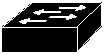
\includegraphics{switch.pdf}};
            \node at (0,-0.6) {#2};
        \end{tikzpicture}
    }
}


\title{STPViz}
\subtitle{Visualizing network topologies with the help of the Spanning Tree Protocol}
\author{Alexander Schlögl}

\begin{document}
\begin{frame}[plain]
    \maketitle
\end{frame}

\begin{frame}{Überblick}
    \begin{itemize}
        \item \textbf{Einleitung \& Motivation}
        \item \textbf{Zeitplanung}
        \item \textbf{Spanning Tree Protocol (STP)}
        \item \textbf{STPViz}
        \item \textbf{Software-Switch}
        \item \textbf{Tests}
        \item \textbf{Zusammenfassung \& Ausblick}
    \end{itemize}
\end{frame}

\begin{frame}{Einleitung \& Motivation}
    \begin{itemize}
        \item Warum STP?
        \item Was ist das Problem?
        \item Was macht STPViz besser/einfacher?
    \end{itemize}
\end{frame}

\begin{frame}{Broadcast Storms}
    \centering
    \begin{tikzpicture}
        \node (root) at (4,8) {\switch{0.8}{A}};
        \node (B) at (2,6) {\switch{0.8}{B}};
        \node (C) at (6,6) {\switch{0.8}{C}};
        \node (D) at (4,4) {\switch{0.8}{D}};

        \draw
        [onslide=<2>{green, thick, ->},
        onslide=<4>{green,thick, <-},
        onslide=<5>{red,thick,<->}]
        (root) edge (B);

        \draw
        [onslide=<2>{green, thick, ->},
        onslide=<4>{green,thick, <-},
        onslide=<5>{red,thick,<->}]
        (root) edge (C);

        \draw
        [onslide=<3>{red, thick, <->},
        onslide=<5>{red, thick, <->}]
        (B) edge (C);

        \draw
        [onslide=<3>{green, thick, ->},
        onslide=<4-5>{red,thick,<->}]
        (B) edge (D);

        \draw
        [onslide=<3>{green, thick, ->},
        onslide=<4-5>{red,thick,<->}]
        (C) edge (D);
    \end{tikzpicture}
\end{frame}

\begin{frame}{Timeline}
    \begin{itemize}
        \item Geplante Timeline
        \item Echte Timeline (mit Problemen)
    \end{itemize}
\end{frame}

\begin{frame}{Spanning Tree Protocol}
    \begin{itemize}
        \item Funktionsweise
        \item Pakete
    \end{itemize}
\end{frame}

\begin{frame}{STP Pakete}
    \centering
    \begin{tikzpicture}[scale=0.35]
        \foreach \x in {0,...,31}
        \node at (\x+0.5,20.5) {\scriptsize \x};
        \draw (0,20) rectangle (16,18.5); \node (mode) at (8, 19.25) {Protocol Identifier};
        \draw (16,20) rectangle (24,18.5); \node (mode) at (20, 19.25) {Version Id};
        \draw (24,20) rectangle (32,18.5); \node (mode) at (28, 19.25) {BPDU Type};
        \draw[onslide=<2>{red,line width=3pt}] (0,18.5) rectangle (8,17); \node (mode) at (4, 17.75) {Flags};
        \draw[onslide=<3>{red,line width=3pt}] (8,18.5) rectangle (32,17); \node (mode) at (20, 17.75) {Root Identifier};
        \draw[onslide=<3>{red,line width=3pt}] (0,17) rectangle (32,15.5); \node (mode) at (16, 16.25) {Root Identifier};
        \draw[onslide=<3>{red,line width=3pt}] (0,15.5) rectangle (8,14); \node (mode) at (4, 14.75) {Root Identifier};
        \draw[onslide=<4>{red,line width=3pt}] (8,15.5) rectangle (32,14); \node (mode) at (20, 14.75) {Root Path Cost};
        \draw[onslide=<4>{red,line width=3pt}] (0,14) rectangle (8,12.5); \node (mode) at (4, 13.25) {Root Path Cost};
        \draw[onslide=<5>{red,line width=3pt}] (8,14) rectangle (32,12.5); \node (mode) at (20, 13.25) {Bridge Identifier};
        \draw[onslide=<5>{red,line width=3pt}] (0,12.5) rectangle (32,11); \node (mode) at (16, 11.75) {Bridge Identifier};
        \draw[onslide=<5>{red,line width=3pt}] (0,11) rectangle (8,9.5); \node (mode) at (4, 10.25) {Bridge Identifier};
        \draw (8,11) rectangle (24,9.5); \node (mode) at (16, 10.25) {Port Identifier};
        \draw[onslide=<6>{red,line width=3pt}] (24,11) rectangle (32,9.5); \node (mode) at (28, 10.25) {Message Age};
        \draw[onslide=<6>{red,line width=3pt}] (0,9.5) rectangle (8,8); \node (mode) at (4, 8.75) {Message Age};
        \draw (8,9.5) rectangle (24,8); \node (mode) at (16, 8.75) {Max Age};
        \draw (24,11) rectangle (32,8); \node (mode) at (28, 8.75) {Hello Time};
        \draw (0,8) rectangle (8,6.5); \node (mode) at (4, 7.25) {Hello Time};
        \draw (8,8) rectangle (24,6.5); \node (mode) at (16, 7.25) {Forward Delay};
    \end{tikzpicture}
\end{frame}

\begin{frame}{STPViz}
    \begin{itemize}
        \item Struktur \& Funktionsweise
        \item Probleme
        \item Fehlerkorrektur
        \item Darstellung
    \end{itemize}
\end{frame}

\begin{frame}{STP Pakete}
    \centering
    \begin{tikzpicture}[scale=0.35]
        \foreach \x in {0,...,31}
        \node at (\x+0.5,20.5) {\scriptsize \x};
        \draw (0,20) rectangle (16,18.5); \node (mode) at (8, 19.25) {Protocol Identifier};
        \draw (16,20) rectangle (24,18.5); \node (mode) at (20, 19.25) {Version Id};
        \draw (24,20) rectangle (32,18.5); \node (mode) at (28, 19.25) {BPDU Type};
        \draw (0,18.5) rectangle (8,17); \node (mode) at (4, 17.75) {Flags};
        \draw[red, line width=2pt] (8,18.5) rectangle (32,17); \node (mode) at (20, 17.75) {Root Identifier};
        \draw[red, line width=2pt] (0,17) rectangle (32,15.5); \node (mode) at (16, 16.25) {Root Identifier};
        \draw[red, line width=2pt] (0,15.5) rectangle (8,14); \node (mode) at (4, 14.75) {Root Identifier};
        \draw (8,15.5) rectangle (32,14); \node (mode) at (20, 14.75) {Root Path Cost};
        \draw (0,14) rectangle (8,12.5); \node (mode) at (4, 13.25) {Root Path Cost};
        \draw[blue, line width=2pt] (8,14) rectangle (32,12.5); \node (mode) at (20, 13.25) {Bridge Identifier};
        \draw[blue, line width=2pt] (0,12.5) rectangle (32,11); \node (mode) at (16, 11.75) {Bridge Identifier};
        \draw[blue, line width=2pt] (0,11) rectangle (8,9.5); \node (mode) at (4, 10.25) {Bridge Identifier};
        \draw (8,11) rectangle (24,9.5); \node (mode) at (16, 10.25) {Port Identifier};
        \draw[green, line width=2pt] (24,11) rectangle (32,9.5); \node (mode) at (28, 10.25) {Message Age};
        \draw[green, line width=2pt] (0,9.5) rectangle (8,8); \node (mode) at (4, 8.75) {Message Age};
        \draw (8,9.5) rectangle (24,8); \node (mode) at (16, 8.75) {Max Age};
        \draw (24,11) rectangle (32,8); \node (mode) at (28, 8.75) {Hello Time};
        \draw (0,8) rectangle (8,6.5); \node (mode) at (4, 7.25) {Hello Time};
        \draw (8,8) rectangle (24,6.5); \node (mode) at (16, 7.25) {Forward Delay};
    \end{tikzpicture}
\end{frame}

\begin{frame}{Visualisierung}
    \centering
    \begin{tikzpicture}[nodes=draw]
        \node[circle, onslide=<2-3>{red}, onslide=<4-6>{white},onslide=<7>{red},onslide=<8>{black}] (r) at (16,10) {};

        \node[circle,onslide=<3-5>{white},onslide=<6>{red}] (a0) at (13, 9) {};
        \node[other] (a1) at (15.5, 9) {};
        \node[other] (a2) at (18, 9) {};

        \node[other] (b0) at (12, 8) {};
        \node[circle,onslide=<3-4>{white},onslide=<5>{red}] (b1) at (13.7, 8) {};
        \node[other] (b2) at (14.5, 8) {};
        \node[other] (b3) at (16, 8) {};
        \node[other] (b4) at (17, 8) {};
        \node[other] (b5) at (19, 8) {};

        \node[circle,onslide=<3>{white},onslide=<4>{red}] (c0) at (13, 7) {};
        \node[other] (c1) at (15, 7) {};
        \node[other] (c2) at (17, 7) {};
        \node[other] (c3) at (18, 7) {};

        \node[circle] (d0) at (13.5, 6) {};
        \node[other] (d1) at (15.5, 6) {};
        \node[other] (d2) at (17, 6) {};

        \draw[onslide=<2-3>{white}]
        (d0) -- (c0);

        \draw[onslide=<2-4>{white}]
        (c0) -- (b1);

        \draw[onslide=<2-5>{white}]
        (b1) -- (a0);

        \draw[onslide=<2-6>{white}]
        (a0) -- (r);

        \draw[other, onslide=<2>{white}]
        %stp links
        (r) -- (a1)
        (r) -- (a2)
        
        (a0) -- (b0)
        (a0) -- (b2)

        (a1) -- (b3)

        (a2) -- (b4)
        (a2) -- (b5)

        (b3) -- (c1)

        (b4) -- (c2)

        (b5) -- (c3)

        (c2) -- (d1)

        (c3) -- (d2);

        \draw[white, onslide=<1>{black}]
        %other links
        (a0) -- (b3)
        (a2) -- (b3)
        (b0) -- (c0)
        (b2) -- (c0)
        (b3) -- (c2)
        (c2) -- (c3)
        (c1) -- (d1)
        (b2) -- (c1)
        (c1) -- (d0);
    \end{tikzpicture}
\end{frame}

\begin{frame}{Software-Switch}
    \begin{itemize}
        \item Grund
        \item Funktionsweise
        \item Grenzen \& Beschränkungen
    \end{itemize}
\end{frame}

\begin{frame}{Testing}
    \begin{itemize}
        \item Setup
        \item Physisches Setup
        \item Tests
        \item Resultate
    \end{itemize}
\end{frame}

\begin{frame}{Zusammenfassung und Ausblick}
    \begin{itemize}
        \item STPViz Fähigkeiten
        \item STPViz Grenzen
        \item Software-Switch
        \item Sonstige Dinge (OpenWrt, dd-wrt)
    \end{itemize}
\end{frame}

\begin{frame}{Message}
Ich hätte gerne, dass Zuseher folgendes mit nach Hause nehmen:\\
\begin{itemize}
    \item Information aus STP zu extrahieren ist schwer, da es nur lokales Wissen benutzt.
    \item Wir haben es trotzdem geschafft (nur halt nicht mit maximaler Informationsdichte).
    \item Es gibt nicht viele Use Cases, aber es gibt sie.
    \item STPViz ist eine gute Grundlage für weitere Arbeiten.
\end{itemize}
\end{frame}

\end{document}
